\documentclass[12pt, letterpaper, twoside]{article}
\usepackage[utf8]{inputenc}
\usepackage{graphicx}
\usepackage{hyperref}
\usepackage{subcaption}

\title{Pepper Waiter HRI Project}
\author{Daniele Appetito Salvatore Cognetta Simone Rossetti}
        
\date{September 2021}

\begin{document}

\begin{titlepage}
\maketitle
\end{titlepage}

\tableofcontents

\newpage
    
\newpage
\section{Introduction}

Human Robot Interaction is the study of how one or more humans work with one robots in order to accomplish a goal. The Pepper Waiter project was devised to create such an interaction. 

\

Pepper is a robot created by Softbank Robotics specifically to interact with people. It has tactile, visual, and audio sensors on its head to help a person convey  information in a variety of ways. On top of that it is equipped with an android tablet on its "chest" that can be used for further interaction. 

\

In this project we decided to create a program that allowed to use the Pepper in a bar or restaurant to take an order instead of a human. This idea came to us by thinking of the current global situation and how the less human-to-human contact there is, the better. As such we decided to create a way to adere to the social distancing norms by removing interaction with a human waiter. 

\


\




\section{Inspiration and Research}

For this projec

copy papers + parts of presentations ad justify them to the 

\section{Solution}

talk about what we decided to do to solve the proposed problem

\section{Implementation}
Different tools and API are used in order to create human interactions with a Pepper real robot or simulator, like:

\begin{itemize}
	\item Softbank SDK;
	\item Naoqi softwares;
	\item MODIM - Multi-modalInteraction Manager.
\end{itemize}

All of the tools are described in the following paragraphs.\\

\subsection{Softbank SDK simulator}
The Softbank company, which produces Pepper robots, has made avaible an SDK which allows to connect to a real robot or to create a simulation of the robot using Android Studioa application (\href{https://qisdk.softbankrobotics.com/sdk/doc/pepper-sdk/index.html}{Softbank SDK}). Because of Covid constraints, it was not possible to use directly the Pepper robot, placed in the laboratories of DIAG-University of La Sapienza: for this reason the simulatotion mode is was used.\\

This simulator gives the opportunity of visualize the movements, the dialogs and the interactions that the robot has with people.

\begin{figure}[htbp]
	\centerline{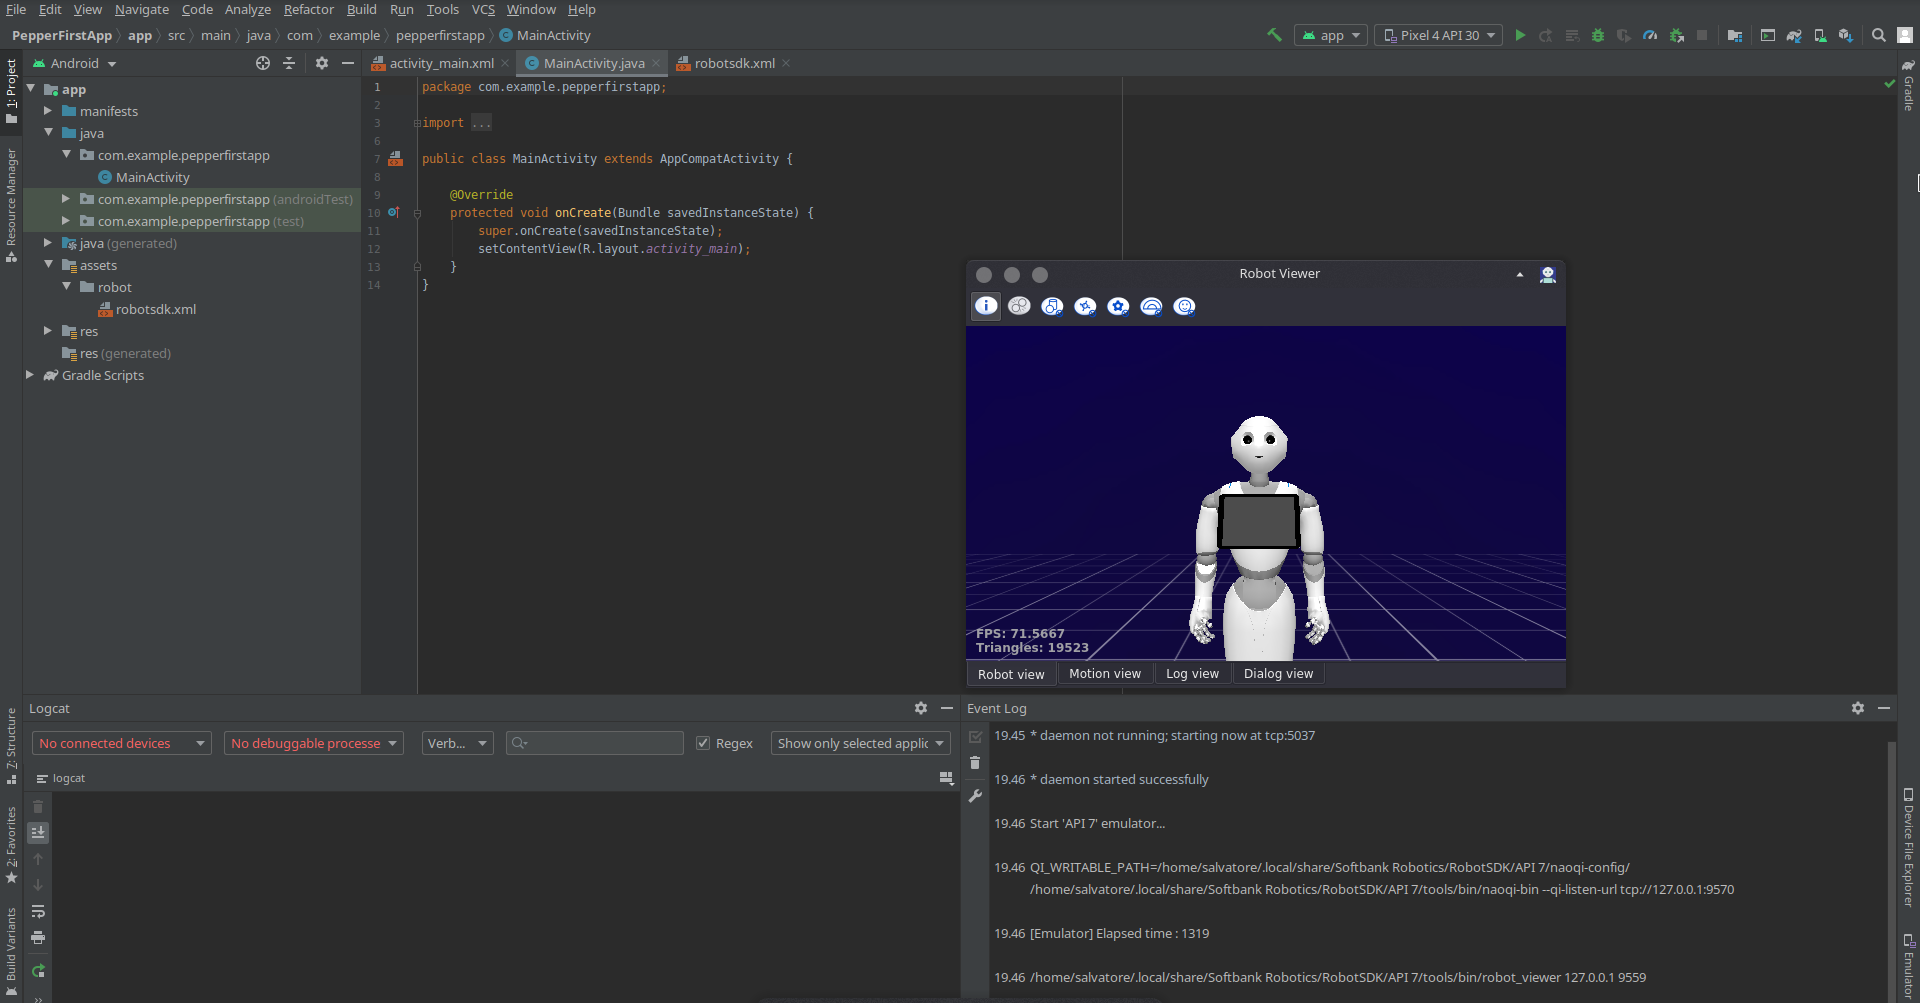
\includegraphics[scale=.3]{img/pepperSDK.png}}
	\caption{Pepper simulator in Android Studio.}
	\label{fig:android_sdk}
\end{figure}

Therefore, to be able to interact and communicate with Pepper, this simulator is used as a client interface, which is connected to a docker image containing the \verb|naoqi| Operative System, containing all the tools and softwares used to run and operate the robot itself.\\
In the simulator, as can be seen from the figure \ref{fig:android_sdk}, there is also a tablet on the chest of the robot. This tablet can be virtualized through another library, modim, later detailed.

\subsection{Naoqi - Pepper tools}
As said before, the OS of Pepper is virtualized thanks to a docker image that is running on our host systems (For further references see the following \href{https://bitbucket.org/iocchi/hri_software/src/master/}{Git Repository}).\\
Once inside the docker image the \verb|naoqi| software must be started in order to initialize and register all services of Pepper, like Dialogs, TextToSpeech, SpeechRecognitrion and more.\\

\begin{figure}[htbp]
	\centerline{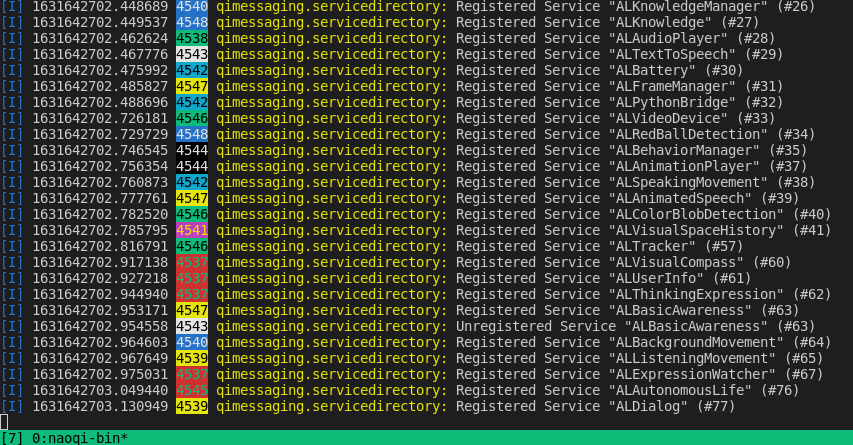
\includegraphics[scale=.6]{img/naoqi.png}}
	\caption{Naoqi SDK: overview of service registered on start.}
	\label{fig}
\end{figure}

This gives us the possibility of command Pepper, indeed inside the docker image different tools are present, with wich one can set some robot parameters like joint angles and the posture, or simulate an input on a sensor like the approach of an human being or a person that talks with Pepper.\\

Beyond the already presented tools, obviously scripts created from us can be runned inside naoqi, in order to set the behaviour of the robot. These scripts can be put inside a shared falder between the host system and the docker image (the directory is \verb|/home/pc_name/playground|). Inside this directory the Pepper Waiter softwares are positioned and developed .

\subsection{Modim}
Like described before, the app running on Pepper's tablet can be virtualized through antoher library called Modim (For further references see the following \href{https://bitbucket.org/mtlazaro/modim.git}{Git Repository})\\

\begin{figure}[htbp]
	\centerline{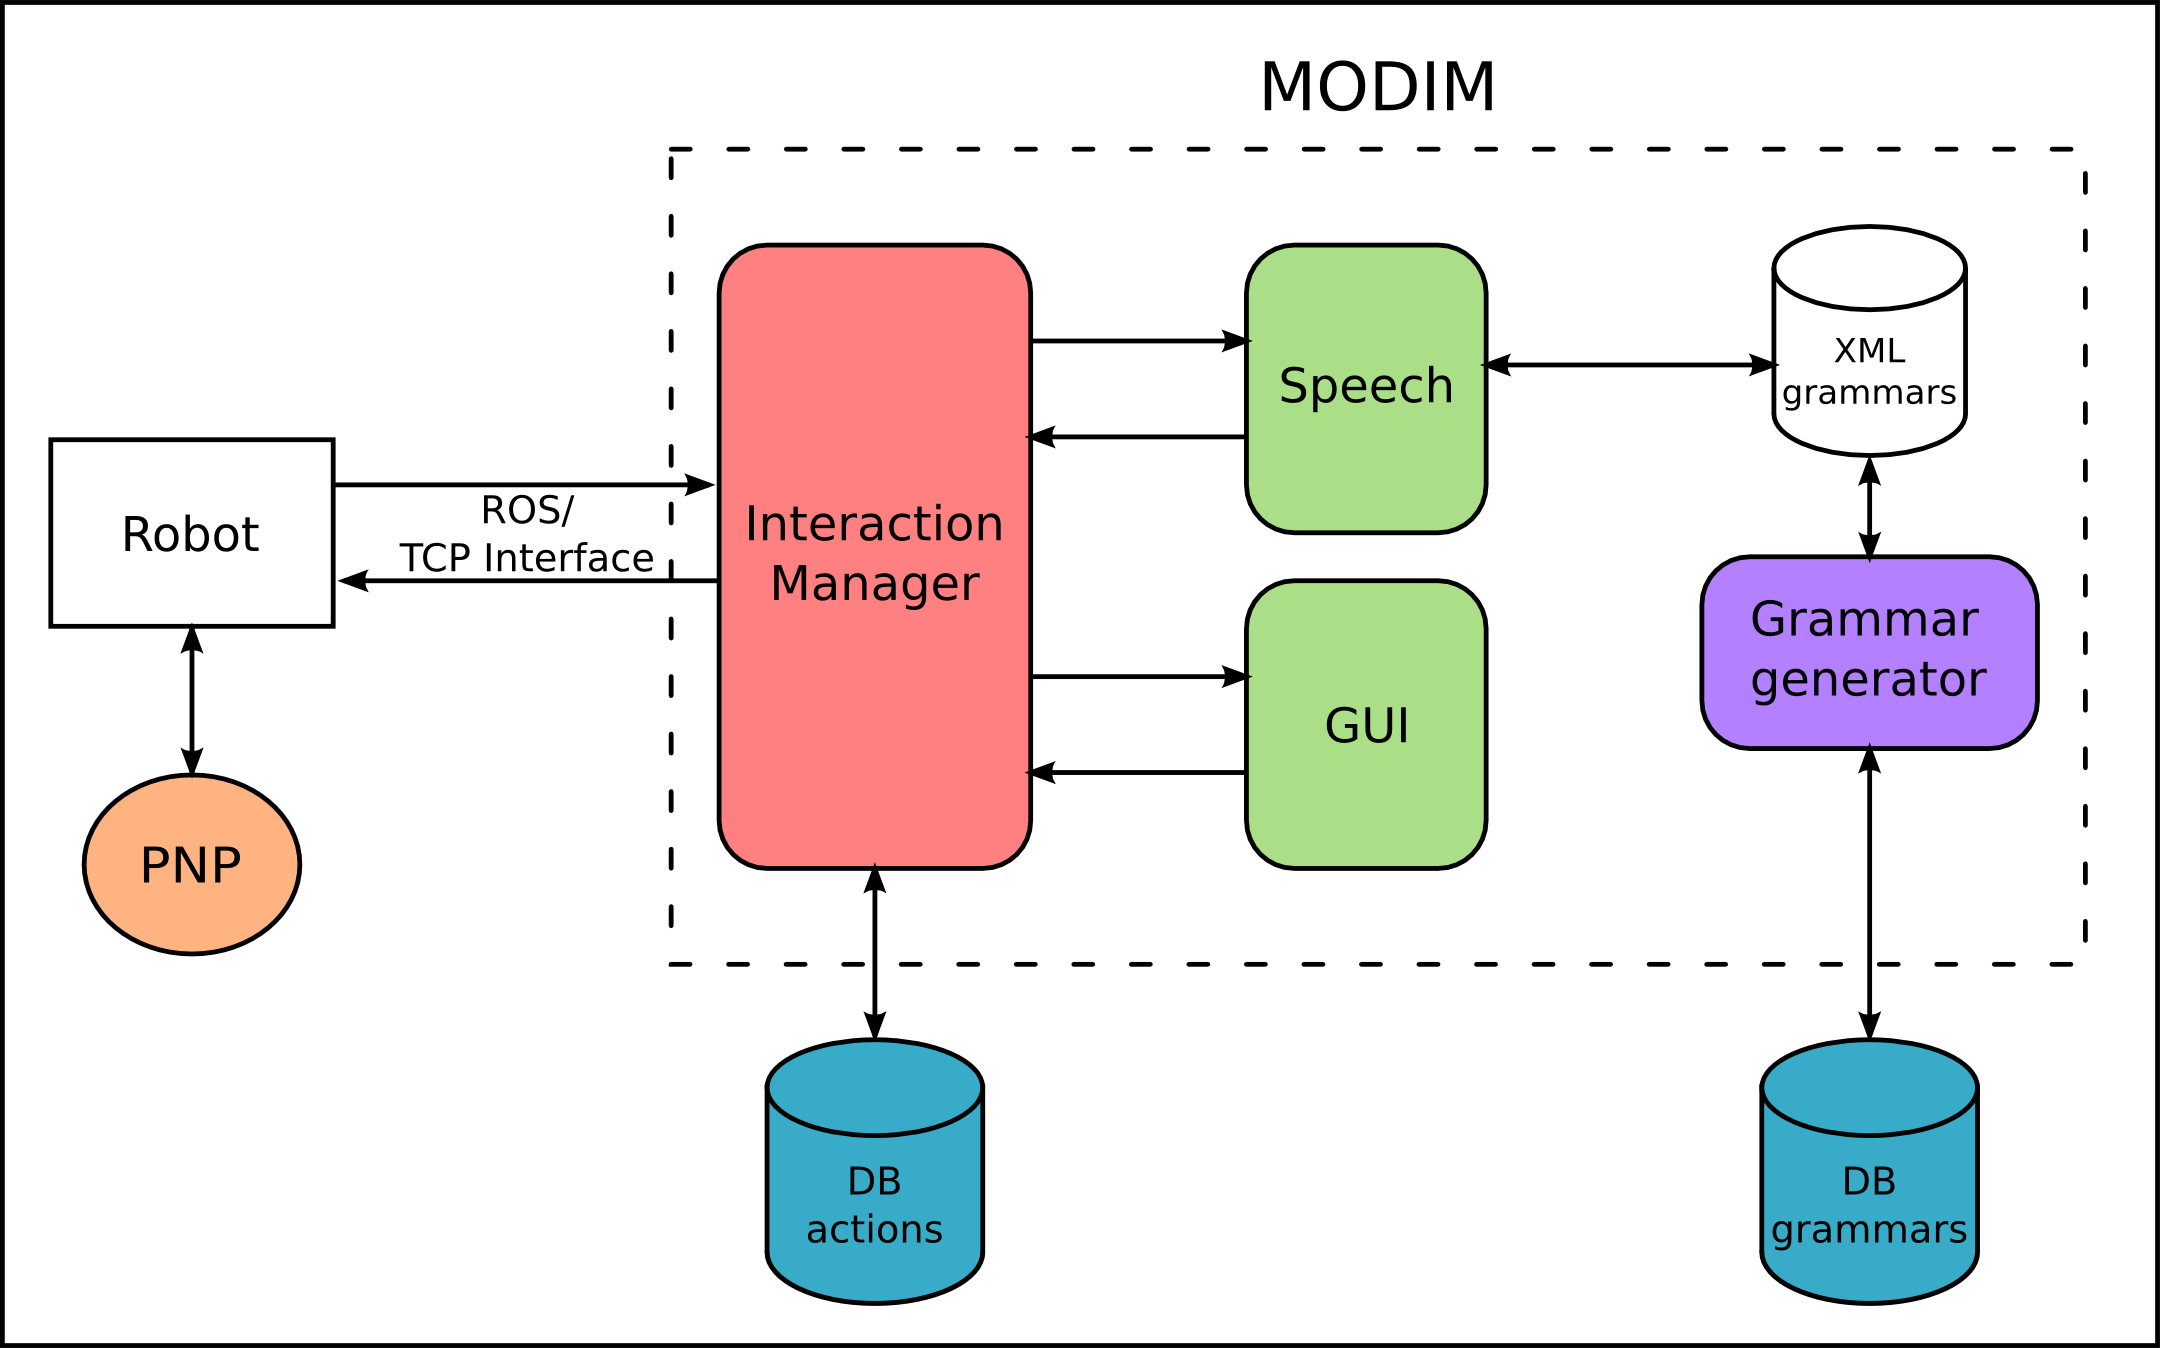
\includegraphics[scale=.6]{img/modim.png}}
	\caption{ Multi-modal Interaction Manager software architecture.}
	\label{fig}
\end{figure}

The Multi-modalInteraction Manager (MODIM), the Graphical User Interface (GUI) and the speech system allow the use of different modalities for the output and input of information from the robot to the user and viceversa. The output modalities considered are the use of texts, images or videos using the GUI or by voice using the speech synthesis. Input modalities are the touch-screen (i.e., with the use of buttons on the GUI) or spoken inputs interpreted by the speech recognizer.\\

Therefore, after connecting the Interatcion Manager with Pepper, thanks to this library the app on the tablet can be simulated on a web browser; the user can interact with this one with buttons present on the GUI, both clickng on them through the web browser and giving spoken input (e.g. simulating them thanks to the \verb|naoqi| software).

\begin{figure}[h]
	\centering
	\begin{subfigure}{.5\textwidth}
	  \centering
	  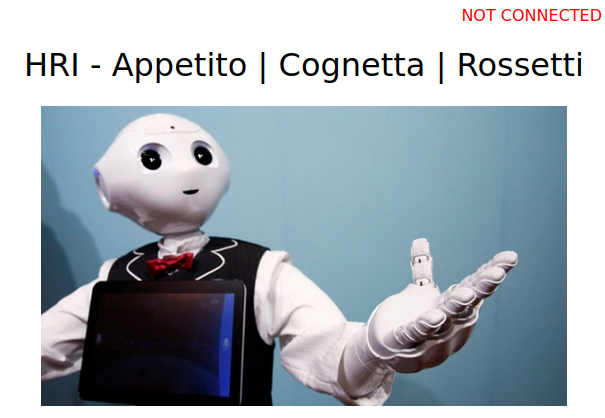
\includegraphics[width=1\linewidth]{img/modim_notok.png}
	  \caption{Modim not connected to Pepper.}
	  \label{fig:sub1}
	\end{subfigure}%
	\begin{subfigure}{.5\textwidth}
	  \centering
	  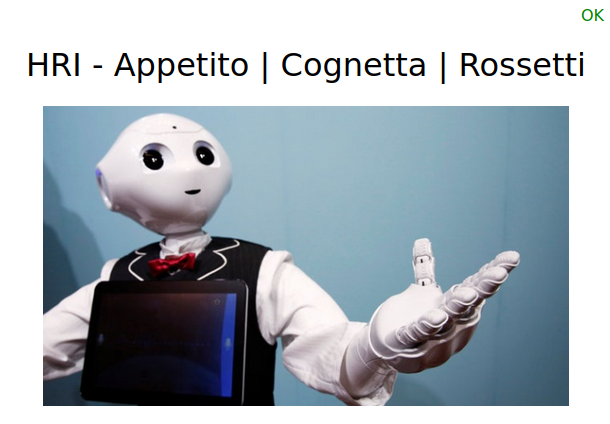
\includegraphics[width=1\linewidth]{img/modim_ok.png}
	  \caption{Modim connected to Pepper.}
	  \label{fig:sub2}
	\end{subfigure}
	\caption{Connection of MODIM to the robot}
	\label{fig:test}
\end{figure}

\newpage

\section{Results}

mini description of functionality

\section{Conclusion}

Conclusion

\end{document}